% Intersección de subespacios: rectas y planos en R3.
\documentclass[compacto,10pt]{pubciencias-notas}
\usepackage{comandosEPN}
\usepackage{tikz}
\usetikzlibrary{babel}
\autor{Departamento de Formación Básica}
\materia{Álgebra Lineal}
\nota{Semana 07 Clase 01}
\fecha{Semestre 2026-B}
\logouno[1.1cm]{Logo_EPN.eps}
\logodos[1.7cm]{Logo_DFB.eps}
\definecolor{colordef}{cmyk}{0.81,0.62,0.00,0.22}
\raggedbottom

\begin{document}
\encabezado
\vspace*{-8mm}
\setcounter{section}{3}
\section{Espacios vectoriales}
\subsection{Rectas y planos en el espacio}

En la semana 06 usamos el criterio de subespacio: contener al cero y ser
cerrado bajo suma y producto por cualquier escalar real. Ahora estudiaremos
qué ocurre cuando imponemos simultáneamente dos restricciones geométricas.
Todas las operaciones de esta clase son las usuales.

\begin{defi}[Recta y plano que pasan por el origen]
    Una recta de $\R^3$ que pasa por el origen $(0,0,0)$ tiene la forma
    \[
        L=\{td:t\in\R\},\qquad d\in\R^3,\quad d\ne0.
    \]
    El vector $d$ indica su dirección y $t$ recorre todos los reales.
    Un plano de $\R^3$ que pasa por el origen tiene la forma
    \[
        P=\{(x,y,z)\in\R^3:ax+by+cz=0\},
    \]
    donde $a,b,c$ son reales no todos nulos.
    Ambos conjuntos son subespacios de $\R^3$.
\end{defi}

\begin{advertencia}
    Una recta o un plano que no contienen al origen no son subespacios
    con las operaciones usuales. Por ejemplo, el plano de ecuación
    $x-y=1$ no contiene a $(0,0,0)$ y, por tanto, no es un subespacio
    de $\R^3$.
\end{advertencia}

\subsection{Intersección: cumplir las dos condiciones}

\begin{defi}[Intersección de subespacios]
    Si $U,W$ son subespacios de un mismo espacio vectorial real $V$,
    su intersección es
    \[
        U\cap W=\{v\in V:v\in U\ \text{y}\ v\in W\}.
    \]
    Un vector de la intersección satisface simultáneamente las condiciones
    de ambos subespacios.
\end{defi}

\begin{teo}
    La intersección de dos subespacios de $V$ es un subespacio de $V$.
\end{teo}

\begin{ejem}[Intersección de dos planos]
    Sean $P$ y $Q$ los subespacios de $\R^3$ dados por
    \[
        P=\{(x,y,z)\in\R^3:x-y=0\},\qquad
        Q=\{(x,y,z)\in\R^3:y-z=0\}.
    \]
    Determine el subespacio $P\cap Q$, escriba sus elementos en forma
    paramétrica e interprete geométricamente el resultado.

    \textbf{Solución.} Un vector pertenece a $P\cap Q$ si satisface
    simultáneamente las condiciones de ambos subespacios. Resolvemos el
    sistema homogéneo
    \[
        \left\{\begin{aligned}x-y&=0,\\y-z&=0.\end{aligned}\right.
        \qquad
        \left(\begin{array}{ccc|c}1&-1&0&0\\0&1&-1&0\end{array}\right).
    \]
    La matriz de coeficientes $A$ y la matriz ampliada $(A\mid0)$ satisfacen
    \[
        \rang(A)=\rang(A\mid0)=2<3,
    \]
    así, el sistema tiene infinitas soluciones
    y una variable libre. Tomando $z=t$, obtenemos $y=t$ y $x=t$. Así,
    \[
        \boxed{P\cap Q=\{(t,t,t):t\in\R\}=\{t(1,1,1):t\in\R\}.}
    \]
    No es un único punto: es la recta completa que pasa por el origen y tiene dirección
    $(1,1,1)$. Por ejemplo, $(2,2,2)$ pertenece a ambos planos.
\end{ejem}

\begin{center}
    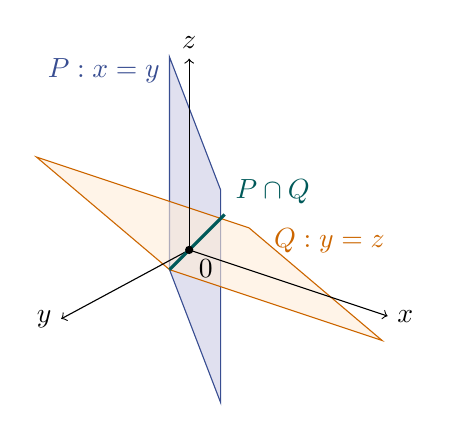
\begin{tikzpicture}[x={(0.9cm,-0.3cm)},y={(-0.65cm,-0.35cm)},z={(0cm,0.9cm)}]
        \filldraw[fill=colordef!12,draw=colordef]
            (-1,-1,-1)--(1.6,1.6,-1)--(1.6,1.6,2)--(-1,-1,2)--cycle;
        \filldraw[fill=orange!15,draw=orange!80!black,fill opacity=0.6]
            (-1,-1,-1)--(2,-1,-1)--(2,1.6,1.6)--(-1,1.6,1.6)--cycle;
        \draw[->] (0,0,0)--(2.8,0,0) node[right] {$x$};
        \draw[->] (0,0,0)--(0,2.5,0) node[left] {$y$};
        \draw[->] (0,0,0)--(0,0,2.7) node[above] {$z$};
        \draw[very thick,teal!70!black] (-1,-1,-1)--(1.8,1.8,1.8)
            node[above right] {$P\cap Q$};
        \fill (0,0,0) circle (1.5pt) node[below right] {$0$};
        \node[colordef,left] at (-1,-1,1.8) {$P:x=y$};
        \node[orange!80!black,right] at (2,1.3,1.3) {$Q:y=z$};
    \end{tikzpicture}
\end{center}

\noindent\textbf{Procedimiento para calcular una intersección.}
\begin{enumerate}
    \item Escribir juntas las condiciones de los dos subespacios.
    \item Resolver el sistema resultante, sin eliminar ninguna restricción.
    \item Escribir todos los vectores solución usando parámetros libres.
    \item En los ejemplos de $\R^3$, identificar si la intersección es $\{(0,0,0)\}$, una recta
          o un plano que pasan por el origen,
          y comprobarlo en las condiciones originales.
\end{enumerate}

\begin{ejem}[Intersección de subespacios de matrices]
    En $\Mat[\R]{2}{2}$, sean los subespacios
    \[
        U=\{A\in\Mat[\R]{2}{2}:a_{12}=a_{21}\},\qquad
        W=\{A\in\Mat[\R]{2}{2}:a_{21}=0\}.
    \]
    El primero contiene las matrices simétricas y el segundo, las
    matrices triangulares superiores. Sus condiciones se conservan al
    sumar matrices y multiplicarlas por escalares reales; ambos contienen
    a la matriz nula. Determine $U\cap W$.

    \textbf{Solución.} Escribimos una matriz arbitraria como
    \[
        A=\begin{pmatrix}a&b\\c&d\end{pmatrix},\qquad a,b,c,d\in\R.
    \]
    Para pertenecer a ambos subespacios debe satisfacer simultáneamente
    \[
        \left\{\begin{aligned}b&=c,\\c&=0.\end{aligned}\right.
    \]
    Por tanto, $b=c=0$, mientras que $a$ y $d$ son libres. Así,
    \[
        \boxed{U\cap W=
            \left\{\begin{pmatrix}a&0\\0&d\end{pmatrix}:a,d\in\R\right\}.}
    \]
    La intersección es el subespacio de las matrices diagonales:
    son precisamente las matrices que son simétricas y triangulares
    superiores a la vez.
\end{ejem}

\begin{ejem}[Intersección de subespacios de polinomios]
    En $\Pol_2$, sean los subespacios
    \[
        U=\{p\in\Pol_2:p(0)=0\},\qquad
        W=\{p\in\Pol_2:p(1)=0\}.
    \]
    Determine $U\cap W$.

    \textbf{Solución.} Sea $p(t)=a_0+a_1t+a_2t^2$, con coeficientes
    reales. Pertenecer a la intersección equivale a cumplir
    \[
        \left\{\begin{aligned}
            p(0)=0&\ \Longleftrightarrow\ a_0=0,\\
            p(1)=0&\ \Longleftrightarrow\ a_0+a_1+a_2=0.
        \end{aligned}\right.
    \]
    Para determinar los coeficientes $a_0,a_1,a_2$, debemos resolver el
    sistema de ecuaciones
    \[
        \left\{\begin{aligned}
            a_0&=0,\\
            a_0+a_1+a_2&=0.
        \end{aligned}\right.
    \]
    La matriz de coeficientes $A$ y la matriz ampliada $(A\mid0)$ cumplen
    \[
        \rang(A)=\rang(A\mid0)=2<3.
    \]
    Por tanto, el sistema tiene infinitas soluciones y una variable libre.
    Tomando $a_2=s$, obtenemos $a_0=0$
    y $a_1=-s$. Por tanto,
    \[
        p(t)=-st+st^2=s(t^2-t),\qquad s\in\R,
    \]
    y la intersección es
    \[
        \boxed{U\cap W=\{s(t^2-t):s\in\R\}.}
    \]
    Sus elementos son todos los múltiplos reales del polinomio $t^2-t$,
    incluido el polinomio cero.
\end{ejem}

\begin{obs}[Otras posibilidades en $\R^3$]
    Si una recta y un plano de $\R^3$ pasan por el origen, la recta está
    contenida en el plano o su intersección es únicamente $\{(0,0,0)\}$.

    Si dos planos distintos de $\R^3$ pasan por el origen, su intersección
    es una recta que también pasa por el origen. Si los planos coinciden,
    su intersección es ese mismo plano.

    Si dos rectas distintas de $\R^3$ pasan por el origen, su único
    punto común es $(0,0,0)$; es decir, su intersección es $\{(0,0,0)\}$.
\end{obs}

\begin{advertencia}
    \textbf{Intersección y unión son diferentes.}
    La unión no siempre es un subespacio. Los ejes coordenados
    \[
        X=\{(t,0,0):t\in\R\},\qquad
        Y=\{(0,t,0):t\in\R\},
    \]
    donde el parámetro $t$ recorre todos los números reales, son
    subespacios de $\R^3$. Sin embargo,
    $(1,0,0)+(0,1,0)=(1,1,0)$ no pertenece a $X\cup Y$.
    En cambio, $X\cap Y=\{(0,0,0)\}$ sí es un subespacio.
\end{advertencia}

\newpage
\section{Ejercicios}

\begin{ejer}[Intersección de planos]
    En $\R^3$, sean
    \[
        P=\{(x,y,z)\in\R^3:x+y-z=0\},\qquad
        Q=\{(x,y,z)\in\R^3:x-y=0\}.
    \]
    \begin{enumerate}
        \item Plantee el sistema que define $P\cap Q$, analice su rango
              y escriba la intersección en forma paramétrica.
        \item Interprete geométricamente el resultado y compruebe un
              vector no nulo en las ecuaciones de ambos planos.
    \end{enumerate}
\end{ejer}

\begin{ejer}[Intersección de subespacios de matrices]
    En $\Mat[\R]{2}{2}$, sean
    \[
        U=\{A\in\Mat[\R]{2}{2}:a_{12}=a_{21}\},\qquad
        W=\{A\in\Mat[\R]{2}{2}:a_{11}=a_{22}\}.
    \]
    \begin{enumerate}
        \item Escriba una matriz arbitraria e imponga las condiciones
              de ambos subespacios. Determine $U\cap W$ mediante
              parámetros reales.
        \item Elija una matriz no nula de la intersección y compruebe
              que pertenece tanto a $U$ como a $W$.
    \end{enumerate}
\end{ejer}

\begin{ejer}[Intersección de subespacios de polinomios]
    En $\Pol_2$, sean
    \[
        U=\{p\in\Pol_2:p(1)=0\},\qquad
        W=\{p\in\Pol_2:p(-1)=0\}.
    \]
    \begin{enumerate}
        \item Escriba $p(t)=a_0+a_1t+a_2t^2$, plantee el sistema en
              los coeficientes y analice su rango. Determine $U\cap W$
              mediante parámetros reales.
        \item Compruebe un polinomio no nulo de la intersección evaluándolo
              en 1 y en $-1$.
    \end{enumerate}
\end{ejer}

\begin{ejer}[Interpretar la intersección]
    Justifique sus respuestas usando que la intersección es un subespacio.
    \begin{enumerate}
        \item ¿Puede la intersección de dos subespacios ser vacía?
        \item Si la intersección tiene un solo elemento, ¿cuál debe ser?
              Dé un ejemplo de dos subespacios de $\R^2$ con esa intersección.
    \end{enumerate}
\end{ejer}

\end{document}
